\documentclass[12pt,a4paper]{article}

\usepackage[a4paper, margin=1in]{geometry}
\usepackage{graphicx}
\usepackage{float}
\usepackage{listings}
\usepackage{xcolor}
\usepackage{setspace}

\onehalfspacing

\title{\textbf{Introduction to Vision and Robotics LAB}}
\begin{document}

\maketitle

% =========================================================
% LAB 1
% =========================================================

\section{Lab 1: Raster versus Vector Graphics}

\subsection{Objectives}

\begin{itemize}
    \item To understand the difference between raster and vector graphics.
    \item To create a simple SVG logo and export it as a PNG image.
    \item To compare the scalability and quality of SVG and PNG images.
    \item To analyse differences in file size and editability between raster and vector formats.
\end{itemize}

\subsection{Introduction}

Raster and vector graphics represent images differently. Raster graphics store images as pixels while vector graphics use mathematical shapes and paths. Raster images are commonly used for photographs because they can represent detailed colour information, while vector graphics are mainly used for logos, icons and illustrations due to their scalability.

In this lab, an SVG logo was created manually and exported as a PNG image. Both formats were then enlarged and compared in order to observe differences in sharpness, editability and file size. The experiment demonstrates how vector graphics maintain image quality during scaling while raster graphics become pixelated when enlarged.

\subsection{Procedure}

\begin{enumerate}
    \item A new SVG file named \texttt{logo.svg} was created using vs code.
    
    \item SVG elements including a rectangle, circle and text were added manually using SVG markup.
    
    \item The SVG file was opened in a browser to confirm correct rendering.
    
    \item The SVG image was exported as a PNG image named \texttt{logo.png}.
    
    \item Both the SVG and PNG images were inserted into a document at different sizes.
    
    \item The images were enlarged and compared visually to observe differences in quality.
    
    \item File sizes for both image formats were recorded.
\end{enumerate}

\subsection{SVG Code Used}

\begin{lstlisting}[language=HTML, basicstyle=\ttfamily\small, frame=single]

<svg width="300" height="300" viewBox="0 0 300 300"
xmlns="http://www.w3.org/2000/svg">

<rect width="300" height="300" rx="35" fill="#EFEAF7"/>

<circle cx="150" cy="120" r="65" fill="#502D78"/>

<text x="150" y="230" text-anchor="middle"
font-size="36" font-family="Arial" fill="#1E4178">
SU
</text>

</svg>

\end{lstlisting}

\subsection{Results}

The SVG and PNG images were successfully created and compared at different scales.

\subsubsection{Image Comparison}


\begin{figure}[H]
    \centering
    
\includegraphics[width=0.9\linewidth]{Comparison.png}
    \caption{Comparison of enlarged SVG and PNG images}
\end{figure}

The SVG image remained sharp after enlargement while the PNG image became pixelated and slightly blurry.

\subsubsection{File Size and Feature Comparison}

% Replace the sample file sizes with your actual values

\begin{table}[H]
\centering
\caption{Comparison between SVG and PNG formats}
\begin{tabular}{|c|c|c|c|}
\hline
\textbf{Format} & \textbf{File Size} & \textbf{Scalability} & \textbf{Editability} \\
\hline
SVG & 313 Bytes & Can scale without quality loss & Easy to edit using code \\
\hline
PNG & 8.30 KB & Loses quality when enlarged & Requires image editing tools \\
\hline
\end{tabular}
\end{table}

\subsection{Discussion}

The experiment showed clear differences between raster and vector graphics. The SVG image maintained smooth edges and sharp text after enlargement because it stores geometric drawing instructions instead of pixels. The browser therefore redraws the image whenever the size changes.

The PNG image became blurry and pixelated when enlarged because raster images contain a fixed number of pixels. Enlarging the image stretches these pixels beyond their original dimensions, reducing image quality.

The SVG file was also easier to edit because the contents could be modified directly in a text editor. In contrast, editing the PNG image would require image editing software. The results therefore show that vector graphics are more suitable for logos and illustrations while raster graphics are better suited for photographs and detailed images.

\subsection{Questions}

\subsubsection{Which version is better for a university logo on a banner? Explain.}

The SVG version is more suitable for a university logo on a banner because it can be enlarged without losing image quality. The logo remains sharp and clear even at very large sizes.

\subsubsection{Which version would be more suitable for a photograph? Explain.}

The PNG version is more suitable for photographs because raster graphics can represent detailed colour variations and textures more effectively than vector graphics.

\subsubsection{Why must SVG be rasterised before being displayed on a screen?}

Computer screens display images using pixels. Since SVG stores mathematical drawing instructions instead of pixels, the browser must first convert the vector shapes into pixels before displaying the image.

\subsection{Sources of Error}

\begin{itemize}
    \item Screenshot compression may slightly affect image quality.
    
    \item Browser rendering differences may affect appearance slightly.
    
    \item PNG export settings may influence file size and image quality.
\end{itemize}

\subsection{Conclusion}

The objective of the lab was successfully achieved by comparing raster and vector graphics using SVG and PNG formats. The experiment showed that SVG images maintain sharpness when enlarged while PNG images lose quality due to pixelation. SVG files were also easier to edit and generally smaller in size for simple graphics. Based on the observations made, vector graphics are more suitable for logos and illustrations while raster graphics are more appropriate for photographs.

\subsection{References}

\begin{enumerate}
    \item R. Steinmetz and K. Nahrstedt, \textit{Multimedia Systems}. Berlin, Germany: Springer, 2004, pp. 112--118.
    
    \item D. F. Rogers, \textit{Procedural Elements for Computer Graphics}, 2nd ed. New York, NY, USA: McGraw-Hill, 1998, pp. 45--52.
    
    \item World Wide Web Consortium, ``Scalable Vector Graphics (SVG) 2 Specification.'' [Online]. Available: https://www.w3.org/TR/SVG2/
\end{enumerate}
\newpage


% =========================================================
% LAB 2
% =========================================================

\section{Lab 2: Image Representation and File Size}

\subsection{Objectives}
\begin{itemize}
    \item To inspect image dimensions, colour mode and channels using Python.
    \item To compare compressed image size with estimated uncompressed raster size.
    \item To understand how image properties affect storage requirements.
    \item To calculate raster image sizes manually.
\end{itemize}

\subsection{Introduction}

Digital images are stored as raster data consisting of pixels arranged in rows and columns. The storage size of an image depends on its dimensions, number of channels and bit depth. Images may also be compressed to reduce storage space and improve transmission efficiency.

In this lab, different images were analysed using Python to inspect their properties and compare compressed file sizes with estimated uncompressed raster sizes. Manual calculations were also performed to understand how image dimensions and colour channels affect storage requirements.

\subsection{Procedure}

\begin{enumerate}
    \item Three images were selected: a photograph, a screenshot containing text and a logo image.
    
    \item A Python script using the Pillow library was executed on each image.
    
    \item The script extracted image properties including dimensions, colour mode and number of channels.
    
    \item Compressed file size and estimated uncompressed size were recorded.
    
    \item Compression ratios for the images were calculated and compared.
    
    \item Manual calculations for raster image storage sizes were performed.
\end{enumerate}

\subsection{Python Code Used}

\begin{lstlisting}[language=Python, basicstyle=\ttfamily\small, frame=single]

from PIL import Image
from pathlib import Path

paths = ["photo.jpg", "screenshot.png", "logo.png"]

for name in paths:
    path = Path(name)
    img = Image.open(path)

    width, height = img.size
    channels = len(img.getbands())

    compressed = path.stat().st_size

    raw_estimate = width * height * channels

    print("\nFile:", name)
    print("Format:", img.format)
    print("Mode:", img.mode)
    print("Dimensions:", width, "x", height)
    print("Channels:", channels)
    print("Compressed size:", compressed, "bytes")
    print("Estimated uncompressed size:", raw_estimate, "bytes")

    print("Approx compression ratio:",
          round(raw_estimate / compressed, 2))

\end{lstlisting}

\subsection{Results}

The Python script successfully extracted image properties and estimated raster sizes.

\subsubsection{Python Output}

\begin{figure}[H]
    \centering
    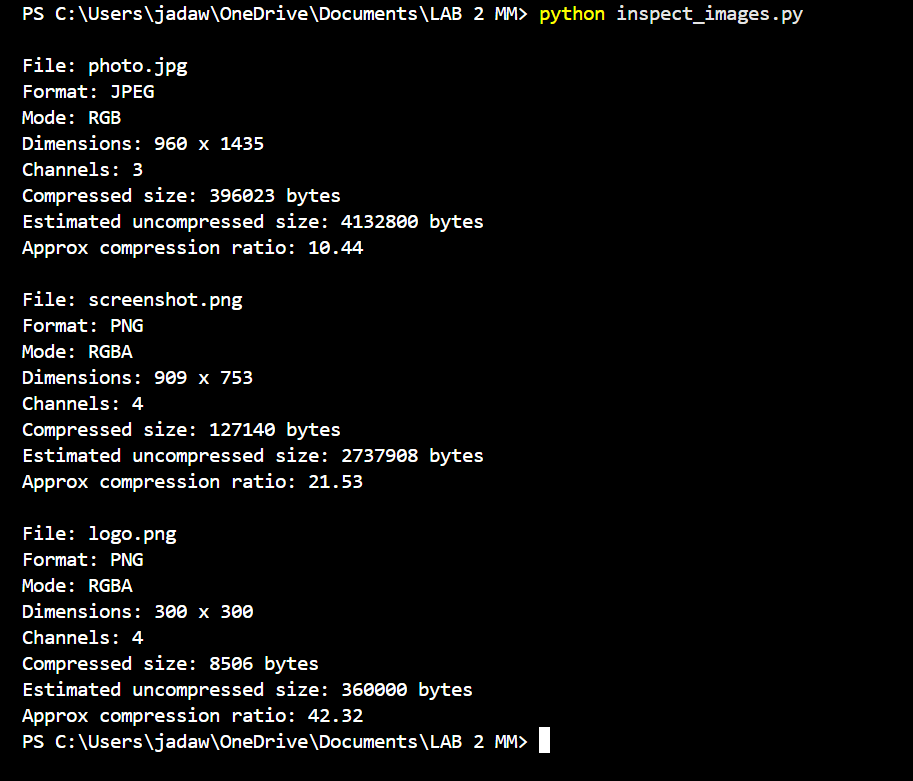
\includegraphics[width=0.9\linewidth]{Lab2_output.png}
\begin{figure}
        \centering
    \end{figure}
        \caption{Python output for image analysis}
\end{figure}

\subsubsection{Compressed vs Uncompressed Size Comparison}

\begin{table}[H]
\centering
\caption{Comparison of compressed and estimated uncompressed sizes}
\begin{tabular}{|c|c|c|c|}
\hline
\textbf{Image} & \textbf{Compressed Size} & \textbf{Estimated Raw Size} & \textbf{Compression Ratio} \\
\hline
photo.jpg & 396.023 KB & 4132.8 KB & 10.44 \\
\hline
screenshot.png & 127.14 KB & 2737.908 KB & 21.53\\
\hline
logo.png & 8506 bytes & 360 KB & 42.32 \\
\hline
\end{tabular}
\end{table}

\subsubsection{Manual Calculations}

\paragraph{1. 1024 × 768 grayscale, 8 bits per pixel}

\[
S = \frac{1024 \times 768 \times 1 \times 8}{8}
\]

\[
S = 786,432 \text{ bytes}
\]

\[
S \approx 768 \text{ KB}
\]

\paragraph{2. 1920 × 1080 RGB, 8 bits per channel}

\[
S = \frac{1920 \times 1080 \times 3 \times 8}{8}
\]

\[
S = 6,220,800 \text{ bytes}
\]

\[
S \approx 5.93 \text{ MB}
\]

\paragraph{3. 3840 × 2160 RGBA, 8 bits per channel}

\[
S = \frac{3840 \times 2160 \times 4 \times 8}{8}
\]

\[
S = 33,177,600 \text{ bytes}
\]

\[
S \approx 31.64 \text{ MB}
\]

\paragraph{4. 4000 × 3000 RGB, 16 bits per channel}

\[
S = \frac{4000 \times 3000 \times 3 \times 16}{8}
\]

\[
S = 72,000,000 \text{ bytes}
\]

\[
S \approx 68.66 \text{ MB}
\]

\subsection{Discussion}

The experiment demonstrated that compressed image sizes are significantly smaller than estimated uncompressed raster sizes. This occurs because image compression algorithms reduce redundant information within the image data.

The screenshot and logo images achieved higher compression ratios because they contained large areas of similar colours and simple patterns. In contrast, the photograph had a lower compression ratio due to its detailed textures and colour variations.

The results also showed that increasing image dimensions, channels or bit depth increases storage requirements. Images containing alpha channels require additional storage because transparency information must also be stored for each pixel.

These observations explain why image compression is important for efficient storage and web delivery. Without compression, image files would require significantly more bandwidth and storage space.

\subsection{Questions}

\subsubsection{Why does adding an alpha channel increase file size?}

An alpha channel stores transparency information for each pixel. This adds an extra channel to the image data, increasing the amount of information stored per pixel and therefore increasing file size.

\subsubsection{Why can two images with the same pixel dimensions have different compressed file sizes?}

Different images contain different amounts of detail, colour variation and repeated patterns. Images with simple patterns compress more efficiently than highly detailed images, leading to different compressed file sizes even when dimensions are identical.

\subsubsection{Why is uncompressed image storage inefficient for web delivery?}

Uncompressed images require large amounts of storage space and bandwidth. This increases loading times and network usage, making compressed formats more suitable for efficient web delivery.

\subsection{Sources of Error}

\begin{itemize}
    \item Compression ratios may vary depending on image content.
    
    \item Different image formats use different compression algorithms.
    
    \item File metadata may slightly affect compressed file size.
\end{itemize}

\subsection{Conclusion}

The lab successfully demonstrated how image dimensions, colour channels and bit depth affect raster image storage size. The Python analysis showed that compressed image files are much smaller than estimated uncompressed raster sizes due to compression techniques. The experiment also showed that image content influences compression efficiency. Overall, the lab highlighted the importance of image compression for storage and web applications.

\subsection{References}

\begin{enumerate}
    \item R. Steinmetz and K. Nahrstedt, \textit{Multimedia Systems}. Berlin, Germany: Springer, 2004, pp. 120--128.
    
    \item D. Salomon, \textit{Data Compression: The Complete Reference}, 4th ed. London, U.K.: Springer, 2007, pp. 85--102.
    
    \item Python Software Foundation, ``Pillow Documentation.'' [Online]. Available: https://pillow.readthedocs.io/
\end{enumerate}
\newpage
% =========================================================
% LAB 3
% =========================================================


\section{Lab 3: Image Formats and Compression Artefacts}

\subsection{Objectives}

\begin{itemize}
    \item To compare JPEG and PNG behaviour on photographs and screenshots.
    \item To observe compression artefacts at different JPEG quality levels.
    \item To analyse the suitability of image formats for different multimedia applications.
\end{itemize}

\subsection{Introduction}

Different image formats use different compression techniques which affect file size and image quality. JPEG is a lossy compression format that reduces file size by removing visually less important information, making it suitable for photographs. PNG is a lossless format that preserves all image data and is commonly used for screenshots, logos and diagrams.

In this lab, JPEG images were exported at different quality levels and compared with PNG versions in order to observe compression artefacts and evaluate format suitability.

\subsection{Procedure}

\begin{enumerate}
    \item A photograph and a screenshot containing text were selected.
    \item Each image was exported as JPEG at quality levels 95, 75, 50 and 20.
    \item Each image was also exported as PNG.
    \item File sizes were recorded for all outputs.
    \item Images were zoomed to 200\% and above to observe compression artefacts.
    \item Screenshots of visible artefacts were captured for analysis.
\end{enumerate}

\subsection{Results}

\subsubsection{File Size and Observation Table}

\begin{table}[H]
\centering
\caption{JPEG vs PNG file sizes and observed artefacts}

\begin{tabular}{|c|c|c|c|}
\hline
\textbf{Image} & \textbf{Format} & \textbf{File Size} & \textbf{Observations} \\
\hline
Photo & JPEG 95 & 500 KB & Almost no artefacts \\
Photo & JPEG 75 & 304 KB & Slight softening \\
Photo & JPEG 50 & 149 KB & Visible compression blocks \\
Photo & JPEG 20 & 48 KB & Strong artefacts and blur \\
Photo & PNG & 2233 KB & No loss in quality \\
\hline
Screenshot & JPEG 95 & 111 KB & Minor edge softening \\
Screenshot & JPEG 75 & 55 KB & Text distortion visible \\
Screenshot & JPEG 50 & 39 KB & Mosquito noise around text \\
Screenshot & JPEG 20 & 25KB & Severe text degradation \\
Screenshot & PNG & 113 KB & Sharp and clear text \\
\hline
\end{tabular}
\end{table}

\subsubsection{Compression Artefacts}

\begin{figure}[H]
    \centering
    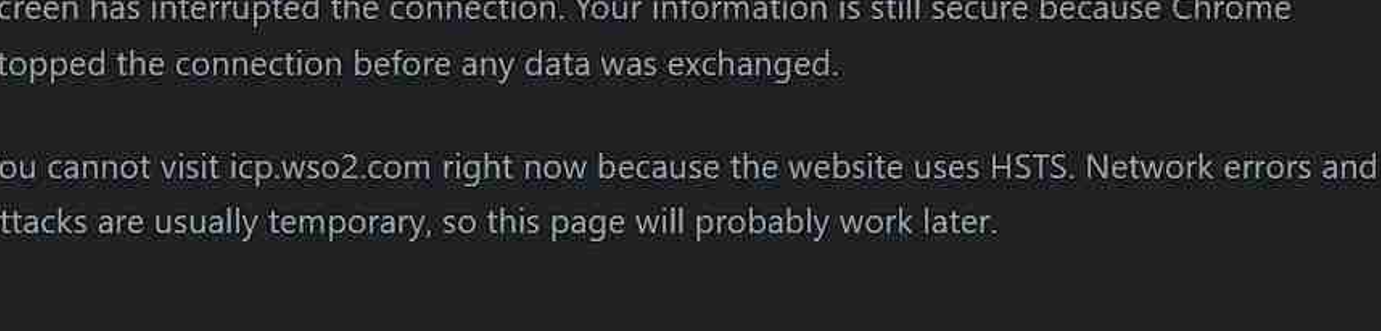
\includegraphics[width=0.9\linewidth]{lab3_artefact1.png}
    \caption{Compression artefacts in JPEG image (screenshot text)}
\end{figure}

\begin{figure}[H]
    \centering
    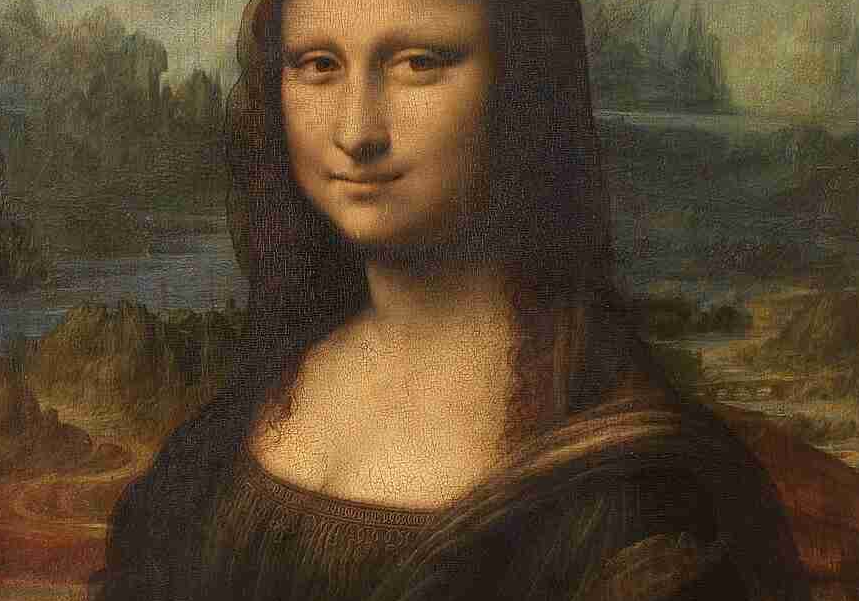
\includegraphics[width=0.9\linewidth]{lab3_artefact2.png}
    \caption{Compression artefacts in JPEG image (photograph)}
\end{figure}

\subsection{Discussion}

The results show that JPEG compression quality significantly affects image clarity. At high quality (95), images remain visually similar to the original. As quality decreases, artefacts such as blockiness, ringing, and loss of fine detail become more visible.

Photographs tolerate JPEG compression better because they contain gradual colour changes and natural textures. Screenshots are more sensitive because they contain sharp edges and text, which are degraded by lossy compression. PNG images remain clear in both cases because they use lossless compression.

These observations confirm that format selection depends on image content and intended use.

\subsection{Questions}

\subsubsection{Why does JPEG usually work better for photographs than screenshots with text?}

JPEG is designed for continuous-tone images such as photographs. It compresses smooth colour transitions efficiently, while sharp edges in text are degraded, causing visible artefacts.

\subsubsection{Why is PNG a strong choice for diagrams and transparent logos?}

PNG uses lossless compression, preserving sharp edges and exact pixel values. This makes it suitable for diagrams, logos and images requiring transparency.

\subsubsection{Why should repeated JPEG editing be avoided?}

Repeated saving of JPEG images introduces cumulative loss of data due to lossy compression. This leads to progressive degradation known as generation loss.

\subsection{Conclusion}

The lab demonstrated that JPEG compression quality directly affects image clarity and artefact visibility. PNG consistently preserved image quality, especially for text-based images. The results confirm that JPEG is more suitable for photographs while PNG is better for screenshots, logos and diagrams.

\subsection{References}

\begin{enumerate}
    \item R. Steinmetz and K. Nahrstedt, \textit{Multimedia Systems}. Springer, 2004.
    \item D. Salomon, \textit{Data Compression: The Complete Reference}. Springer, 2007.
\end{enumerate}
\newpage
% =========================================================
% LAB 4
% =========================================================

\section{Lab 4: Colour Models, Alpha and Transparency}

\subsection{Objectives}

\begin{itemize}
    \item To perform alpha compositing using manual calculations.
    \item To implement alpha blending using Python.
    \item To convert RGB values into CMY colour space.
    \item To understand the role of different colour models in imaging systems.
\end{itemize}

\subsection{Introduction}

Colour representation in digital systems depends on the application domain. RGB is an additive model used in screens where light is emitted, while CMY is a subtractive model used in printing. Alpha compositing introduces transparency, allowing images to be blended based on opacity values.

This lab explores alpha blending through both manual computation and Python implementation, as well as basic conversion between RGB and CMY colour models.

\subsection{Procedure}

\begin{enumerate}
    \item Alpha compositing was performed manually using a foreground and background colour with different opacity values.
    \item A Python script was used to generate an alpha blended image.
    \item RGB values were converted into CMY using a simple mathematical relationship.
\end{enumerate}

\subsection{Manual Alpha Compositing}

Given:
\begin{itemize}
    \item Foreground: $C_f = (255, 0, 0)$
    \item Background: $C_b = (0, 0, 255)$
\end{itemize}

\subsubsection{Formula}

\[
C_o = \alpha C_f + (1 - \alpha) C_b
\]

\subsubsection{Case 1: $\alpha = 0.5$}

\[
C_o = (128, 0, 128)
\]

\subsubsection{Case 2: $\alpha = 0.25$}

\[
C_o = (64, 0, 191)
\]

\subsubsection{Case 3: $\alpha = 0.75$}

\[
C_o = (191, 0, 64)
\]

\subsection{Python Alpha Compositing}

\begin{lstlisting}[language=Python, basicstyle=\ttfamily\small, frame=single]

from PIL import Image, ImageDraw

W, H = 400, 250

background = Image.new("RGB", (W, H), (30, 65, 120))
foreground = Image.new("RGBA", (W, H), (0, 0, 0, 0))

draw = ImageDraw.Draw(foreground)
draw.rectangle((80, 50, 320, 200), fill=(255, 80, 40, 128))

combined = Image.alpha_composite(background.convert("RGBA"), foreground)

combined.save("alpha_composite.png")

\end{lstlisting}

\subsubsection{Output Image}

% Upload alpha_composite.png to Overleaf

\begin{figure}[H]
    \centering
    
\includegraphics[width=0.9\linewidth]{alpha_composite.png}
    \caption{Alpha compositing result using Python}
\end{figure}

\subsection{RGB to CMY Conversion}

Given:
\[
(R, G, B) = (0.2, 0.5, 0.9)
\]

\subsubsection{Formula}

\[
C = 1 - R,\quad M = 1 - G,\quad Y = 1 - B
\]

\subsubsection{Result}

\[
(C, M, Y) = (0.8, 0.5, 0.1)
\]

\subsection{Discussion}

The manual alpha compositing demonstrates how transparency affects final pixel values by blending foreground and background colours based on opacity. Higher alpha values result in stronger foreground influence, while lower values allow more of the background to show through.

The Python implementation confirms this blending visually by overlaying a semi-transparent shape on a background image. The resulting output demonstrates how alpha channels are used in modern image compositing.

The RGB to CMY conversion shows the inverse relationship between additive and subtractive colour models. RGB is used for digital displays, while CMY is more suitable for printing systems.

\subsection{Questions}

\subsubsection{What visual problem can occur if alpha edges are mishandled?}

Incorrect handling of alpha edges can cause visible halos or jagged borders, especially when semi-transparent pixels are not properly blended with the background.

\subsubsection{Why are luma-chroma spaces useful in image and video compression?}

Luma-chroma separation allows compression algorithms to reduce colour information more aggressively than brightness information, improving compression efficiency without significantly affecting perceived quality.

\subsubsection{Why can the same RGB numbers look different on different devices?}

Different devices have varying display technologies, calibration settings and colour gamuts, causing the same RGB values to appear differently across screens.

\subsection{Conclusion}

The lab demonstrated how alpha compositing blends images using transparency values and how RGB relates to CMY colour representation. The Python implementation visually confirmed theoretical calculations, and the conversion exercise highlighted differences between additive and subtractive colour models.

\subsection{References}

\begin{enumerate}
    \item R. Steinmetz and K. Nahrstedt, \textit{Multimedia Systems}. Springer, 2004.
    \item W3C, ``Compositing and Blending Level 1.'' https://www.w3.org/TR/compositing-1/
\end{enumerate}
\end{document}